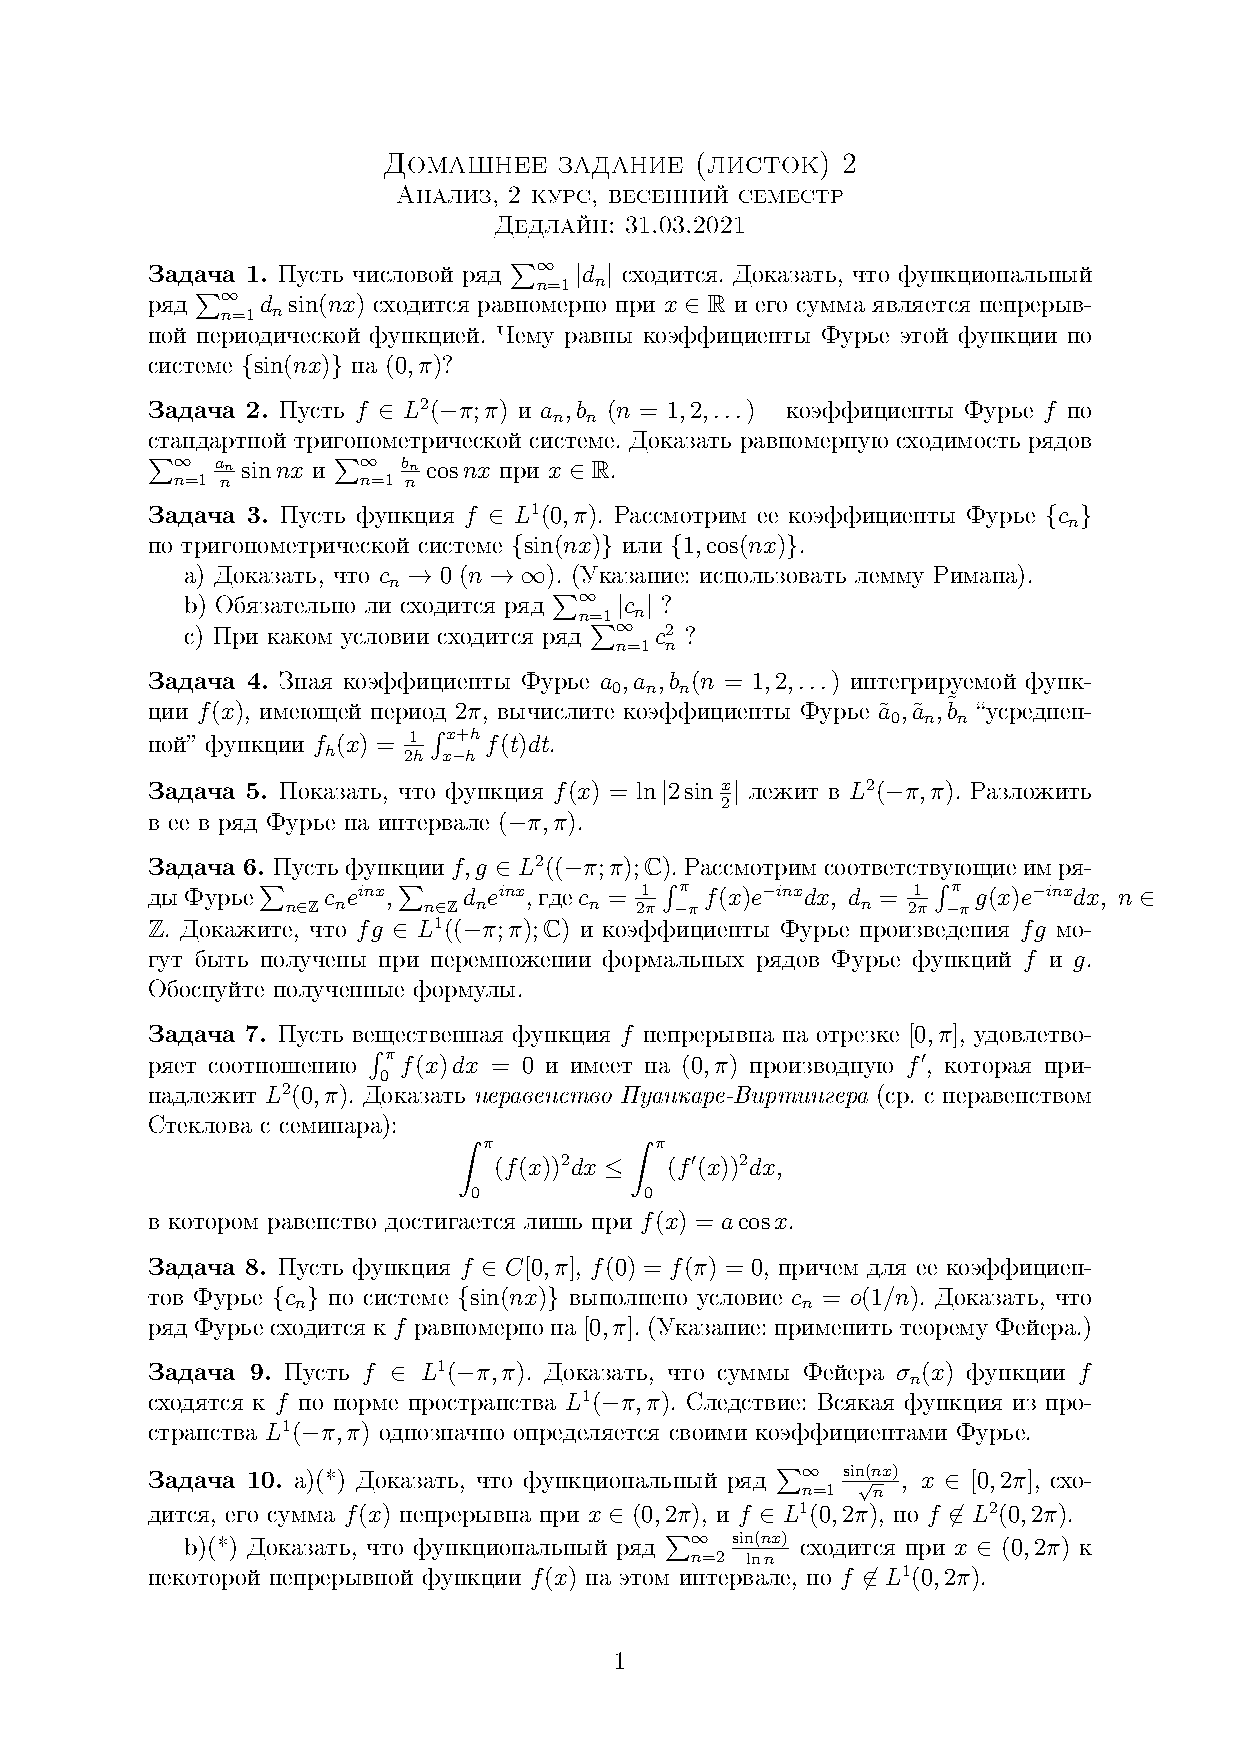
\includepdf[scale=1,pages=1]{Tasks/Listok2_2021.pdf}
\newpage
\section*{Решения}
\subsection*{Задача 1}
	$|\sin(nx)| \leqslant 1 \Rightarrow |d_n||\sin(nx)| \leqslant |d_n|$. Из словия $\sum\limits_{n = 1}^{\infty} |d_n|$ сходится, также $|d_n \sin(nx)| \leqslant |d_n|$, тогда $\sum\limits_{n = 1}^{\infty} |d_n \sin(nx)|$ сходится, а следовательно и $\sum\limits_{n = 1}^{\infty} d_n \sin(nx)$ сходится\\
	Пусть $f = \sum\limits_{n = 1}^{\infty} d_n \sin(nx),\ S_k = \sum\limits_{n = 1}^{k} d_n \sin(nx)$. Докажем, что $\sum\limits_{n = 1}^{\infty} d_n \sin(nx)$ сходится равномерно, то есть $\forall \varepsilon > 0\ \exists K_{\varepsilon}:\ \forall K > K_{\varepsilon}:\ |f - S_K(x)| < \varepsilon$
	\begin{gather*}
		|\sum\limits_{n = 1}^{\infty} d_n \sin(nx) - \sum\limits_{n = 1}^{k} d_n \sin(nx)|
		= |\sum\limits_{n = k+1}^{\infty} d_n \sin(nx)|
		\leqslant \sum\limits_{n = k+1}^{\infty} |d_n \sin(nx)|
		= \sum\limits_{n = k+1}^{\infty} (|d_n| |\sin(nx)|)
		\leqslant \sum\limits_{n = k+1}^{\infty} d_n \cdot 1\\
		|f(x) - S_k(x)| \leqslant \sum\limits_{n = k+1}^{\infty} |d_n|
	\end{gather*}
	Если ряд $\sum a_n$ сходится, то $\lim\limits_{n \to \infty} \sum\limits_{k = n+1}^{\infty} a_k = 0$, применим это к $\sum |d_n|:\ \forall \varepsilon > 0\ \exists N_{\varepsilon}:\ \forall n > N_{\varepsilon}:\ |d_n| < \varepsilon$, откуда $|f - S_k| \leqslant \sum\limits_{n = k+1}^{\infty} |d_n| < \varepsilon$, тогда $|f - S_k(x)| < \varepsilon\ (\forall \varepsilon > 0\ \exists N_{\varepsilon}:\ \forall n > N_{\varepsilon})$, следовательно ряд сходится равномерно
	\vskip 0.1in
	Заметим, что из равномерной сходимости и непрерывности $d_n \sin(nx)$ следует непрерывность $f$, заметим что $f$ периодична $d_k \sin(k (x + 2\pi)) = d_k \sin(kx + k \cdot 2\pi) = d_k \sin(kx) \Rightarrow f(x + 2\pi) = f(x)$\\
	Тогда $f(x) = \sum\limits_{k = 1}^{\infty} b_k \sin(kx),\ b_k = \frac{2}{\pi} \int\limits_{0}^{\pi} f(x) \sin(kx) dx$, тогда
	\begin{gather*}
		\int\limits_{0}^{\pi} \sum d_n \sin(nx) \sin(kx) dx
		= \sum\limits_{k \ne n} \int\limits_{0}^{\pi} d_n \sin(nx) \sin(kx) dx
		+ \int\limits_{0}^{\pi} d_k \sin^2(kx) dx\\
		= \sum \frac{d_n}{2} (\int\limits_{0}^{\pi} \cos(n - k)x dx - \int\limits_{0}^{\pi} \cos(n+k)x dx) + \frac{d_k}{2} \int\limits_{0}^{\pi} (1 - \cos(2kx))dx\\
		= \sum \frac{d_n}{2} (\frac{\sin(n-k)x}{n-k} \bigg|_{0}^{\pi} - \frac{\sin(n+k)x}{n+k} \bigg|_{0}^{\pi}) + \frac{d_k}{2} (x\bigg|_{0}^{\pi} - \frac{\sin(2kx)}{2x}\bigg|_{0}^{\pi})
		= \frac{d_k}{2}\pi\\
		b_k = \frac{2}{\pi} \cdot \frac{d_k \pi}{2} = d_k\qquad
		f(x) = \sum\limits_{k = 1}^{\infty} d_k \sin(kx)
	\end{gather*}
\vskip 0.4in
\begin{comment}
	Пусть $\sum\limits_{n=1}^{\infty} |d_n|$ сходится к $0$. Заметим, что
	\begin{gather*}
		D_n(x) = \sum\limits_{k = 1}^{n} \sin(kx)\\
		2 \sin \frac{x}{2} D_n(x)
		= \sum\limits_{k = 1}^{n} 2\sin \frac{x}{2} \sin(kx)
		= \sum\limits_{k = 1}^{n} \left(\cos((k - \frac{1}{2})x) - \cos((k + \frac{1}{2})x)\right)
		= \cos \frac{x}{2} - \cos((n + \frac{1}{2})x)\\
		|D_n(x)|
		= \left|\frac{\cos \frac{x}{2} - \cos((n + \frac{1}{2})x)}{2\sin \frac{x}{2}}\right|
		\leqslant \frac{1}{|\sin \frac{x}{2}|}
	\end{gather*}
	Тогда если $x \in [\varepsilon, 2\pi - \varepsilon]$, то $\frac{x}{2} \in [\frac{\varepsilon}{2}, \pi - \frac{\varepsilon}{2}]$ и $|D_n(x)| \leqslant \frac{1}{\sin \frac{\varepsilon}{2}}$\\
	Далее мы можем воспользоваться признаком Дирихле, и получить что ряд $\sum\limits_{n=1}^{\infty} d_n \sin(nx)$ сходится
\end{comment}

\subsection*{Задача 2}
	\begin{gather*}
		f(x)
		= \frac{a_0}{2} + \sum\limits_{n = 1}^{\infty} (a_n \sin(nx) + b_n \cos(nx))\\
		a_n = \frac{1}{\pi} \int_{-\pi}^{\pi} f(x) \sin(nx)dx\\
		b_n = \frac{1}{\pi} \int_{-\pi}^{\pi} f(x) \cos(nx)dx
	\end{gather*}
	Если $\{\varphi_n\}$ -- некоторая ортогональная нормированная система в $R$ (не бязательно полная). Из нерваенства Бесселя вытекает, что для того, чтобы числа $c_1, c_2, \ldots$ служили коэффициентами Фурье какого-то элемента $f \in R$, необходимо чтобы ряд $\sum\limits_{k = 1}^{\infty} c_k^2$ сходился.\\
	\begin{gather*}
		a_1^2 + b_1^2 + a_2^2 + b_2^2 + \ldots 
		= \sum\limits_{i = 1}^{n} (a_n^2 + b_n^2)
		= \sum\limits_{i = 1}^{n} a_n^2 + \sum\limits_{i = 1}^{n} b_n^2
	\end{gather*}
	Сходится, а следовательно
	\begin{gather*}
		\sum\limits_{i = 1}^{n} a_n^2,\ \sum\limits_{i = 1}^{n} b_n^2
	\end{gather*}
	Тоже сходятся
	\vskip 0.1in
	\begin{gather*}
		\left(\sum \frac{|a_n|}{n}\right)^2
		= \left(\sum |a_n| \cdot \frac{1}{n}\right)^2
		\leqslant \left(\sum a_n^2\right) + \left(\sum b_n^2 \right)\\
		\sum \frac{|a_n|}{n}
		\leqslant \sqrt{\left(\sum a_n^2 \right) \cdot \left(\sum b_n^2\right)}
	\end{gather*}
	То есть $\sum \frac{a_n}{n}$ сходится, а следовательно по признаку вейерштрасса
	\begin{gather*}
		\left| \frac{a_n \sin(nx)}{n} \right|
		\leqslant \left| \frac{a_n \cdot 1}{n} \right|
		= \frac{a_n}{n}
	\end{gather*}
	То есть $\sum\limits_{n=1}^{\infty} \frac{|a_n|}{n} \sin(nx)$ сходится равномерно.\\
	Аналогично доказывается сходимость $\sum\limits_{n=1}^{\infty} \frac{|b_n|}{n} \cos(nx)$
\vskip 0.4in

\subsection*{Задача 3}
\begin{enumerate}
\item[(a)]
	Воспользуемся леммой Римана, $f \in L^1(0,\pi),\ f \sim \sum\limits_{n \in \mathbb{Z}} c_n e^{inx}$, где $c_n = \frac{1}{2\pi} \int_{0}^{\pi} f(t) e^{-int} dt$ -- коэффициенты Фурье. Рассмотрим частичную сумму 
	\begin{gather*}
	S_n(x)
	= \sum\limits_{|k| \leqslant n} c_k \cdot e^{ikx}
	= \sum\limits_{|k| \leqslant n} \left(\frac{1}{2\pi} \int_{-\pi}^{\pi} f(t) e^{ikt} dt\right) e^{ikx}
	= \int_{-\pi}^{\pi} \frac{f(x)}{2\pi} \left(\sum\limits_{|k| \leqslant n} e^{ik(x-t)}\right)dt\\
	= \frac{1}{\pi} \int_{-\pi}^{\pi} f(t) \frac{\sin \frac{2n+1}{2}(t-x)}{2\sin \frac{t-x}{2}} dt
	= \frac{1}{\pi} \int_{-\pi}^{\pi} f(t) D_n (t-x)dt
	2(f \circ D_n)(x)\\
	D_n(x) = \frac{\sin \frac{2n+1}{2}x}{2\sin \frac{x}{2}}
	\end{gather*}
	Так мы пришли к интегралу Дирихле, сделав замену $t - x = z$ получим
	\begin{gather*}
	S_n(x)
	= \frac{1}{\pi} \int_{-\pi-x}^{\pi-x} f(x+z) D_n(z) dz
	= \frac{1}{\pi} \int_{-\pi}^{\pi} f(x+z) D_n(z) dz\\
	\\
	\frac{1}{\pi} \int_{-\pi}^{\pi} D_n(z)dz
	= \frac{1}{2\pi} \int_{-\pi}^{\pi} \sum\limits_{|k| \leqslant n} e^{ikz} dz
	= 1\\
	\\
	S_n(x) - f(x) = \frac{1}{\pi} \int_{-\pi}^{\pi}(f(x+z) - f(x)) D_n(x)dz
	\end{gather*}
	Сумма ряда Фурье $\sum\limits_{n \in \mathbb{Z}} c_n e^{inx}$ совпадает с пределом интеграла Дирихле при $n \to \infty$.
\item[(b)]
	Рассмотрим $f(x) = x$. $f \in L^1(0,\pi) \Rightarrow$ подходит по условию
	\begin{gather*}
		c_n 
		= \frac{2}{\pi} \int\limits_{0}^{\pi} x \sin(nx) dx 
		= \frac{-2}{\pi n} \int\limits_{0}^{\pi} x d \cos(nx)\\
		= \frac{-2}{\pi n} (x \cos(nx) \bigg|_{0}^{\pi} - \int\limits_{0}^{\pi} \cos(nx) dx)
		= \frac{-2}{\pi n} (\pi \cos(\pi n) - \frac{\sin(nx)}{n}\bigg|_{0}^{\pi})
		= (-1)^{n+1} \frac{2}{n}
	\end{gather*}
	$|c_n| = \frac{2}{n},\ \sum\limits_{n = 1}^{\infty}|c_n| = \sum\limits_{n=1}^{\infty} \frac{2}{n} = 2 \sum\limits_{n=1}^{\infty} \frac{1}{n}$ -- как известно, не сходится
	
\item[(c)]
	Докажем, что $f \in L^2(0,\pi) \Leftrightarrow \sum\limits_{n=1}^{\infty} c_n^2$ сходится.\\
	Из неравенства Бесселя следует, что для того, чтобы числа $c_1, \ldots, c_n, \ldots$ служили коэффициентами Фурье какого-то элемента $f \in E$, необходимо чтобы ряд $\sum\limits_{k = 1}^{\infty} c_k^2$ сходился.\\
	($\Rightarrow$) Если $f \in L^2(0,\pi)$, то так как $\{c_n\}$ -- коэффициенты Фурье $f \in L^2(0,\pi) \subset L^1(0,\pi)$, ряд $\sum\limits_{k=1}^{\infty} c_k^2$ сходится.\\
	($\Leftarrow$) По теореме Рисса если $\sum\limits_{n = 1}^{\infty} c_n^2$ схдится, то в $L^2 (0,\pi)$ есть функция с коэффициентами $\{c_n\}$, а так как функция задается коэффициентами Фурье однозначно, то эта функция и есть наша $f$, откуда $f \in L^2(0,\pi)$
\end{enumerate} 
\vskip 0.4in

\subsection*{Задача 4}
	Сделаем замену $t = x + z,\ z = t - x$
	\begin{gather*}
	c_n(f_n)
	= \frac{1}{2\pi} \int_{-\pi}^{\pi} f_h(x) e^{-inx}dx
	= \frac{1}{2\pi} \int_{-\pi}^{\pi} \left(\frac{1}{2h} \int_{-h}^{h} f(x+z) dz\right)e^{-inx} dx
	= \frac{1}{2\pi \cdot 2h} \int_{-h}^{h} \left(\int_{-\pi}^{\pi} f(x+z)e^{-inx} dx\right)dz\\
	= \frac{1}{2h} \int_{-h}^{h} \left(\frac{1}{2\pi} \int_{-\pi}^{\pi} f(y) e^{-in(y-z)} dy\right) dz
	= \frac{1}{2h} \int_{-h}^{h}\left(\frac{1}{2\pi} \int_{-\pi+z}^{\pi+z} f(y) e^{-in(y-z)} dy\right) dz\\
	= \frac{1}{2h} \int_{-h}^{h} e^{inz} \left(\frac{1}{2\pi} \int_{-\pi+z}^{\pi+z} f(y) e^{-iny} dy\right) dz
	= \frac{1}{2h} \int_{-h}^{h} e^{inz} \left(\frac{1}{2\pi} \int_{-\pi}^{\pi} f(y) e^{-iny} dy\right) dz\\
	= c_n(f) \frac{1}{2h} \int_{-h}^{h} e^{inz} dz
	= c_n(f) \frac{1}{2h} \frac{e^{inz}}{in}\bigg|_{-h}^{h}
	= c_n(f) \frac{1}{nh} \frac{e^{inh} - e^{-inh}}{2i}
	= c_n(f) \frac{\sin nh}{nh}
	\end{gather*}
	Откуда
	\begin{gather*}
	c_n(f_n) = c_n(f) \frac{\sin nh}{nh}
	\end{gather*}
\vskip 0.4in

\subsection*{Задача 5}
	\begin{gather*}
	\ln|2 \sin \frac{x}{2}|
	= \ln|e^{\frac{ix}{2}} - e^{-\frac{ix}{2}}|
	= \ln|\frac{e^{ix} - 1}{e^{\frac{ix}{2}}}|
	= \ln|e^{ix} - 1| - \ln|e^{\frac{ix}{2}}|
	= \ln|e^{ix} - 1|
	\end{gather*}
	Откуда
	\begin{gather*}
	\ln(1+x) = x - \frac{x^2}{2} + \frac{x^3}{3} - \ldots\\
	f(x) = \ln|e^{ix} - 1| = (e^{ix} - 2) - \frac{(e^{ix} - 2)^2}{2} + \ldots
	\end{gather*}
	То есть $f^2(x)$ интегрируема и $\in L_2(-\pi, \pi)$
	Теперь посчитаем
	\begin{gather*}
	\int_{-\pi}^{\pi} \ln|e^{ix} - 1| \cos(nx) dx
	= \frac{1}{n} \int_{-\pi}^{\pi} \ln|2 \sin \frac{x}{2}| d \sin nx
	= -\frac{1}{n} \int_{-\pi}^{\pi} \sin(nx) \frac{\cos \frac{x}{2}}{2\sin \frac{x}{2}} dx\\
	\end{gather*}
	Тогда так как
	\begin{gather*}
	D_n(x) = \frac{1}{2} + \sum\limits_{k = 1}^{n} \cos(kx)
	= \frac{\sin((n + \frac{1}{2})x)}{2\sin \frac{x}{2}}
	= \frac{\sin(nx) \cos \frac{x}{2} + \cos(nx) \sin \frac{x}{2}}{2 \sin \frac{x}{2}}
	\end{gather*}
	То
	\begin{gather*}
	\frac{1}{n} \int_{-\pi}^{\pi}\sin(nx) \frac{\cos \frac{x}{2}}{2 \sin \frac{x}{2}}dx
	= \frac{1}{n} \int_{-\pi}^{\pi}\left(D_n(x) - \frac{\cos(nx) \sin \frac{x}{2}}{2 \sin \frac{x}{2}}\right)dx\\
	\int_{-\pi}^{\pi} D_n(x) = \pi\\
	\int_{-\pi}^{\pi} \frac{\cos(nx) \sin \frac{x}{2}}{2 \sin \frac{x}{2}}dx
	= \int_{-\pi}^{\pi} \frac{\cos(nx)}{2} = 0\\
	-\frac{1}{n} \int_{-\pi}^{\pi} \sin(nx) \frac{\cos \frac{x}{2}}{2 \sin \frac{x}{2}}dx = -\frac{\pi}{n}\\
	||\sin nx||^2 = \int_{-\pi}^{\pi} \sin^2(nx) dx
	= \int_{-\pi}^{\pi} \frac{1}{2} - \frac{\cos(2nx)}{2}dx = \pi 
	\end{gather*}
	Откуда
	\begin{gather*}
	\ln|2 \sin \frac{x}{2}| = -\sum\limits_{k = 1}^{\infty} \frac{\cos(kx)}{k}
	\end{gather*}

\begin{comment}
	Коэффициенты имеют вид:
	\begin{gather*}
		a_0 = \frac{1}{2\pi} \int_{-\pi}^{\pi} f(x)dx\\
		a_n = \frac{1}{\pi} \int_{-\pi}^{\pi} f(x)\cos(nx)dx\\
		b_n = \frac{1}{\pi} \int_{-\pi}^{\pi} f(x)\sin(nx)dx
	\end{gather*}
	Посчитаем $a_n$
	\begin{gather*}
		a_n = \frac{1}{\pi} \int_{-\pi}^{\pi} f(x)\cos(nx)dx
		= \frac{1}{\pi} \int_{-\pi}^{\pi} \ln\left|2\sin \frac{x}{2}\right| \cos(nx)dx\\
		= \frac{1}{\pi} \int_{-\pi}^{\pi} \ln\left|2 \frac{e^{i \frac{x}{2}} - e^{-i \frac{x}{2}}}{2i}\right| \cdot \frac{e^{ixn} + e^{-ixn}}{2}dx
		= \frac{1}{\pi} \int_{-\pi}^{\pi} \ln\left|e^{i \frac{x}{2}} + e^{-i \frac{x}{2}}\right| \cdot \frac{e^{ixn} + e^{-ixn}}{2}dx\\
		= \frac{1}{\pi} 
		\left( 
			\ln\left|e^{i \frac{x}{2}} + e^{-i \frac{x}{2}}\right| \cdot \frac{e^{ixn} + e^{-ixn}}{2}\bigg|_{-\pi}^{\pi}
			-

		\right)
	\end{gather*}
\end{comment}
\vskip 0.4in

\subsection*{Задача 6}
	\begin{gather*}
		\int\limits_{-\pi}^{\pi} |fg|dx
		\leqslant \sqrt{\int_{-\pi}^{\pi} |f|^2} \sqrt{\int_{-\pi}^{\pi} |g|^2}
		= ||f||_2||g||_2
		< \infty\\
		\\
		f(x) = \sum\limits_{n \in \mathbb{Z}} c_n e^{inx}
		= \sum a_n \cos(nx) + b_n \sin(nx)\\
		g(x) = \sum a_n e^{inx}
		= \sum \alpha_n \cos(nx) + \beta_n \sin(nx)\\
		fg = \frac{A_0}{2} + \sum\limits_{m = 1}^{\infty} A_m \cos(mx) + B_m \sin(mx)\\
		c_0 = \frac{a_0}{2}\qquad
		c_n = \frac{a_n - ib_n}{2}\qquad
		c_{-n} = \frac{a_n + ib_n}{2}
	\end{gather*}
	Обобщение формулы Парсеваля - обобщ. уравнение замкнутости: $\frac{1}{\pi}\int\limits_{-\pi}^{\pi} f(x)g(x)dx = \frac{a_0 \alpha_0}{2} + \sum\limits_{m = 1}^{\infty} (a_m \alpha_m + b_m \beta_m)$
	\begin{gather*}
		A_0 = \frac{1}{\pi} \int\limits_{-\pi}^{\pi} fg dx
		= \frac{a_0 \alpha_0}{2} + \sum\limits_{m=1}^{\infty} a_m \alpha_m + b_m \beta_m\\
		A_k = \frac{1}{\pi} \int\limits_{-\pi}^{\pi} fg \cos(kx) dx
	\end{gather*}
	Коэффициенты Фурье для $\phi(x):$
	\begin{gather*}
		\frac{1}{\pi} \int\limits_{-\pi}^{\pi} g(x) \cos(kx) \cos(mx) dx
		= \frac{1}{2} (\frac{1}{\pi} \int\limits_{-\pi}^{\pi} g(x)\cos(m+k)x dx + \frac{1}{\pi}\int\limits_{-\pi}^{\pi}g \cos(m-k)x dx)
		= \frac{1}{2} (\alpha_{m+k} + \alpha_{m-k})\\
		\frac{1}{\pi} \int\limits_{-\pi}^{\pi} g(x) \cos(kx)dx = \alpha_k\\
		\frac{1}{\pi} \int\limits_{-\pi}^{\pi} g(x) \cos(kx) \sin(mx) dx
		= \frac{1}{2} (\beta_{m+k} + \beta_{m-k})\\
		A_k = \frac{1}{\pi} \int\limits_{-\pi}^{\pi} fg \cos(kx) dx
		= \frac{a_0 \alpha_k}{2} + \frac{1}{2}\sum\limits_{m=1}^{\infty} a_m(\alpha_{m+k} + \alpha_{m-k}) + b_m(\beta_{m+k} + \beta_{m-k})\\
		B_k = \frac{a_0 \beta_{k}}{2} + \frac{1}{2} \sum\limits_{m=1}^{\infty} a_m (\beta_{m+k} + \beta_{m-k}) - b_m(\alpha_{m+k} + \alpha_{m-k})\\
		\\
		(\frac{a_0}{2} + \sum\limits_{n=1}^{\infty} a_n \cos(nx) + b_n \sin(nx))(\frac{\alpha_0}{2} + \sum\limits_{n=1}^{\infty} \alpha_n \cos(nx) + \beta_n \sin(nx))\\
		= \frac{a_0 \alpha_0}{4}
		+ \sum\limits_{n=1}^{\infty}(\frac{a_0}{2}\alpha_n + \frac{\alpha_0}{2}a_n)\cos(nx)
		+ \sum\limits_{n=1}^{\infty}(\frac{a_0}{2}\beta_{n} + \frac{\alpha_0}{2}b_n)\sin(nx)\\
		+ \sum\limits_{n=1}^{\infty} a_n \cos(nx) \sum\limits_{k=1}^{\infty} \alpha_k \cos(kx) 
		+ \sum\limits_{n=1}^{\infty} b_n \cos(nx) \sum\limits_{k=1}^{\infty} \alpha_k \cos(kx)\\ 
		+ \sum\limits_{n=1}^{\infty} a_n \cos(nx) \sum\limits_{k=1}^{\infty} \beta_k \cos(kx)
		+ \sum\limits_{n=1}^{\infty} b_n \cos(nx) \sum\limits_{k=1}^{\infty} \beta_k \cos(kx)
	\end{gather*}

\vskip 0.4in

\subsection*{Задача 7}
	Если $a_n$ -- комплексные коэффициенты ряда Фурье для $f$, то у $f'$ коэффициенты имеют вид $ina_n$, тогда применив равенство Парсеваля к $f'$ и используя
	\begin{gather*}
		a_0 = \frac{1}{2\pi} \int\limits_{0}^{2\pi}f(x)dx = 0
	\end{gather*}
	Получим что
	\begin{gather*}
		\frac{1}{2\pi} \int\limits_{0}^{2\pi} f'^{2}(x)dx
		= \sum\limits_{-\infty}^{\infty} n^2 |a_n|^2
		\geqslant \sum\limits_{-\infty}^{\infty} |a_n|^2
		= \frac{1}{2\pi} \int\limits_{0}^{2\pi} f^2(x)dx
	\end{gather*}
\vskip 0.4in

\subsection*{Задача 8}
	(1)\\
	Пусть
	\begin{gather*}
		S_k(x)
		= \sum\limits_{n = 1}^{k} c_n \sin(nx)\\
		\sigma_n = \frac{s_1(x) + \ldots + s_n(x)}{n}
	\end{gather*}
	Необходимо доаказать, что $S_k(x) \rightrightarrows f$ на $[0, \pi]$.\\
	По теореме Фейера $\{\sigma_n\} \rightrightarrows f$ на $[0, \pi]$, 
	\begin{gather*}
		\sigma_n(x)
		= \frac{s_1(x) + \ldots + s_n(x)}{n}
		= \frac{\sum\limits_{k = 1}^{1}c_k \sin(kx) + \sum\limits_{k = 1}^{2}c_k \sin(kx) + \ldots + \sum\limits_{k = 1}^{n}c_k \sin(kx)}{n}
	\end{gather*}
	Заметим что $c_1 \sin(x)$ входит в каждую сумму, $c_2 \sin(2x)$ во все кроме первой, $c_3 \sin(3x)$ во все кроме первых двух и т.д., тогда
	\begin{gather*}
		\sigma_n(x)
		= \frac{c_1 n \sin(x) + c_2 (n-1) \sin(2x) + \ldots + c_n \sin(nx)}{n}\\
		= \frac{n(c_1 \sin(x) + c_2 \sin(2x) + \ldots + c_n \sin(nx)) - c_2 \sin(2x) - \ldots - (n-1) c_n \sin(nx)}{n}\\
		= S_n - \sum\limits_{k = 1}^{n} \frac{k-1}{n} c_k \sin(kx)
		= S_n - \frac{1}{n} \sum\limits_{k = 1}^{n} k c_k \sin(kx)
		+ \frac{1}{n} \sum\limits_{k = 1}^{n} c_k \sin(kx)\\
		= S_n (1 + \frac{1}{n}) - \frac{1}{n} \sum\limits_{k = 1}^{n} k c_k \sin(kx)
	\end{gather*}
	Тогда $\sigma_n(x) = S_n (1 + \frac{1}{n}) - \frac{1}{n} \sum\limits_{k = 1}^{n} k c_k \sin(kx)$
	\vskip 0.1in
	(2)\\
	По условию $c_n = o(\frac{1}{n})$, то есть $\forall a\ \exists N:\ \forall n > N\ |c_n| \leqslant a|\frac{1}{n}| \leftrightarrow |n c_n| \leqslant a$. Заметим, что $|n c_n \sin(nx) \leqslant |n c_n|$, тогда $|n c_n \sin(nx)| \leqslant |n c_n| \leqslant a$. Итак, $|n c_n \sin(nx)| \leqslant a$
	\begin{gather*}
		\forall x \frac{1}{n} |\sum\limits_{k = N + 1}^{n} k c_k \sin(kx)|
		\leqslant \frac{1}{n} \sum\limits_{k = N + 1}^{n} |k c_k \sin(kx)|
		\leqslant \frac{1}{n} \sum\limits_{k = N + 1}^{n} a
		= \frac{1}{n} a(n - N)
		= a (1 - \frac{N}{n})
		= a - a \frac{N}{n}
		< a
	\end{gather*}
	То есть $\forall x\ \frac{1}{n} |\sum\limits_{k = N+1}^{n} kc_k \sin(kx)| < a$, обозначим $\sum\limits_{k = 1}^{N} k c_k \sin(kx)$ как $M$
	\vskip 0.1in
	(3)
	\begin{gather*}
		\forall x\ |\sigma_m (x) - S_n(1 + \frac{1}{n}|
		= |\frac{1}{n} \sum\limits_{k = 1}^{n} k c_k \sin(kx)|
		= \frac{1}{n} |\sum\limits_{k = 1}^{N} k c_k \sin(kx) + \sum\limits_{k = N + 1}^{n} k c_k \sin(kx)|
		< \frac{1}{n} |M + na|
		\leqslant |\frac{M}{n}| + a 
	\end{gather*}
	Пусть $n > N$ и $|\frac{M}{n}| < a$, тогда $|\frac{M}{n}| + a \leqslant 2a \Rightarrow \sigma_n(x) - S_n(1 + \frac{1}{n}) \rightrightarrows f$
	\vskip 0.1in
	(4)\\
	\begin{gather*}
		\forall x\ |f(x) - (1 + \frac{1}{n}) S_n|
		= |f(x) - \sigma_n(x) + \sigma_n(x) - (1 + \frac{1}{n}) S_n|\\
		\leqslant |f(x) - \sigma_n(x)| + |\sigma_n(x) - (1 + \frac{1}{n})S_n|
		< a + 2a
		< 3a\\
		\Rightarrow
		(1 + \frac{1}{n})S_n \rightrightarrows f
	\end{gather*}
	\vskip 0.1in
	(5)\\
	$(1 + \frac{1}{n})S_n = S_n + \frac{1}{n} S_n$. Пусть $\sum\limits_{k = 1}^{N} c_k \sin(kx) = \alpha$. Выберем $n$ достаточно большое, чтобы $|\frac{\alpha}{n}| < a$.
	\begin{gather*}
		|\frac{1}{n} S_n|
		= |\frac{1}{n} \sum\limits_{k = 1}^{n} c_k \sin(kx)|
		= |\frac{1}{n} \sum\limits_{k = 1}^{N} c_k \sin(kx) + \frac{1}{n} \sum\limits_{k = N + 1}^{n} c_k \sin(kx)|\\
		\leqslant |\frac{\alpha}{n}| + \frac{1}{n} \sum\limits_{k = N+1}^{n} a
		= |\frac{\alpha}{n}| + \frac{1}{n} a (n - N)
		= |\frac{\alpha}{n}| + a - \frac{Na}{n}
		< a + a
		= 2a
	\end{gather*}
	Тогда $\forall x\ |f(x) - S_n(x)| = |f(x) - S_n(x) + \frac{1}{n} S_n(x) - \frac{1}{n} S_n(x)| = |(f(x) - (1 + \frac{1}{n})S_n(x)) + \frac{1}{n} S_n(x)| \leqslant 2a + 3a$ (по (4) и (5)), что и требовалось доказать
\vskip 0.4in

\subsection*{Задача 9}
	Продолжим $f$ по $2\pi$-ериодичности на всю ось
	\begin{gather*}
	||f(x) - \sigma_n(x)||
	= \int\limits_{-\pi}^{\pi} |f(x) - \sigma_n(x)| dx
	= \int\limits_{-\pi}^{\pi} |f(x) - \int\limits_{-\pi}^{\pi}f(x+z) \Phi_n(z) dz|dx\\
	= \int\limits_{-\pi}^{\pi} | \int\limits_{-\pi}^{\pi} (f(x) - f(x+z)) \Phi_n(z) dz| dx
	\leqslant \int\limits_{-\pi}^{\pi} \int\limits_{-\pi}^{\pi} |(f(x) - f(x+z))\Phi_n(z)| dz dx\\
	= \int\limits_{-\pi}^{\pi} \int\limits_{-\pi}^{\pi} |f(x) - f(x+z)| \Phi_n(z) dz dx
	= \int\limits_{-\pi}^{\pi} \Phi_n(z) \int\limits_{-\pi}^{\pi} |f(x) - f(x+z)| dx dz\\
	\\
	\lim\limits_{z \to 0} \int\limits_{-\pi}^{\pi} |f(x) - f(x+z)|dx = 0 \Leftrightarrow
	\forall \varepsilon > 0\ \exists \delta: |z| < \delta \Rightarrow
	\int\limits_{-\pi}^{\pi} |f(x) - f(x+z)| dx < \varepsilon\\
	\\
	\int\limits_{-\pi}^{\pi} \Phi_n(z) \int\limits_{-\pi}^{\pi} |f(x) - f(x+z)| dxdz\\
	= \int\limits_{-\pi}^{-\delta} \Phi_n(z) \int\limits_{-\pi}^{\pi} |f(x) - f(x+z)| dxdz
	+ \int\limits_{-\delta}^{\delta} \Phi_n(z) \int\limits_{-\pi}^{\pi} |f(x) - f(x+z)| dxdz
	+ \int\limits_{\delta}^{\pi} \Phi_n(z) \int\limits_{-\pi}^{\pi} |f(x) - f(x+z)| dxdz\\
	= I_{-} + I_{0} + I_{+}
	\end{gather*}
	Заметим что $\int\limits_{-\pi}^{\pi} |f(x) - f(x+z)|dx < \infty$, так как по неравенству Минковского $\int\limits_{-\pi}^{\pi} |f(x) - f(x+z)| \leqslant \int\limits_{-\pi}^{\pi} |f(x)|dx + \int\limits_{-\pi}^{\pi} |f(x+z)|dx < \infty$\\
	Обозначим $\int\limits_{-\pi}^{\pi} |f(x) - f(x+z)|dx$ как $M$\\
	Возьмем $n_0$ настолько большим, что $\eta_n(\delta) < \varepsilon$ при $n > n_0$, тогда
	\begin{gather*}
		I_{-} = \int\limits_{-\delta}^{\pi} \Phi_n(z) M dz = \eta_n (\delta) M < \varepsilon M\\
		I_{0} = \int\limits_{-\delta}^{\delta} \Phi_n(z) M dz < \int\limits_{-\delta}^{\delta} \Phi_n(z) \varepsilon dz < \varepsilon \int\limits_{-\pi}^{\pi} \Phi_n(z)dz < \varepsilon\\
		I_{+} = \int\limits_{-\pi}^{\delta} \Phi_n(z) M dz < \varepsilon M\\
		||f(x) - \sigma_n(x)|| < 2 \varepsilon M + \varepsilon \to 0\quad \text{при } \varepsilon \to 0
	\end{gather*}
\begin{comment}
	Пусть $n$ частичная суммая ряда Фурье это $s_n$, тогда
	\begin{gather*}
		s_n(x) = \sum_{k = -n}^{n} \hat{f}(k)e^{ikx}\\
		\sigma_n(x) = \frac{1}{n+1} \sum_{k = 0}^{n}s_k(x)
	\end{gather*}
	Можно расписать $s_n(x)$ как
	\begin{gather*}
		s_n(x) = \sum\limits_{k = -n}^{n} \hat{f}(k) e^{ikx}
		= \sum\limits_{k = -n}^{n} \left(\frac{1}{2\pi} \int\limits_{-\pi}^{\pi} f(t) e^{-ikt} dt\right) e^{ikt}\\
		= \frac{1}{2\pi} \int\limits_{-\pi}^{\pi} f(t) \sum\limits_{k = -n}^{n} e^{ik(x - t)}dt
		= \frac{1}{2\pi} \int\limits_{-\pi}^{\pi} f(x) D_n(x - t) dt
		= \frac{1}{2\pi} \int\limits_{-\pi}^{\pi} f(x - t) D_n(x) dt
	\end{gather*}
	Тогда $\sigma_n(x)$
	\begin{gather*}
		\sigma_{n}(x)\
		= \frac{1}{n + 1} \sum\limits_{k = 0}^{n} s_k(x)
		= \frac{1}{n + 1} \sum\limits_{k = 0}^{n} \left(\frac{1}{2\pi} \int\limits_{-\pi}^{\pi} f(x - t) D_k(t) dt\right)\\
		= \frac{1}{2\pi} \int\limits_{-\pi}^{\pi} f(x - t) \left(\frac{1}{n+1} \sum\limits_{k = 0}^{n} D_k(t)\right) dt
		= \frac{1}{2\pi} \int\limits_{-\pi}^{\pi} f(x - t) F_n(t) dt
	\end{gather*}
	Откуда
	\begin{gather*}
		\sigma_n(x) - f(x) = \frac{1}{2\pi}\int_{-\pi}^{\pi} (f(x - t) - f(x)) F_n(t) dt
	\end{gather*}
	Тогда по неравенству треугольника
	\begin{gather*}
		|\sigma_n(x) - f(x)| \leqslant \frac{1}{2\pi} \int\limits_{-\pi}^{\pi} |(f(x - t) - f(x)) F_n(t)| dt\\
		|\sigma_n(x) - f(x)| \leqslant \frac{1}{2\pi} \int\limits_{-\pi}^{\pi} |(f(x - t) - f(x))| F_n(t) dt
	\end{gather*}
	Откуда
	\begin{gather*}
		|\sigma_n(x) - f(x)| 
		= \left(\frac{1}{2\pi} \int\limits_{|t| \leqslant \sigma} |f(x - t) - f(x)| F_n(t) dt\right) + \left(\frac{1}{2\pi} \int\limits_{\sigma \leqslant |t| \leqslant \pi} |f(x - t) - f(x)| F_n dt\right) 
	\end{gather*}
	Первый интеграл ограничен сверху
	\begin{gather*}
		\frac{1}{2\pi} \int\limits_{|t| \leqslant \sigma} \varepsilon F_n(t) dt
		\leqslant \frac{1}{2\pi} \int\limits_{-\pi}^{\pi} \varepsilon F_n(t) dt = \varepsilon
	\end{gather*}
	Второй интеграл ограничен
	\begin{gather*}
		\frac{1}{2\pi} \int\limits_{\sigma \leqslant |t| \leqslant \pi} 2 (\sup\limits_{-\pi \leqslant t \leqslant \pi} |f(t)|) F_n(t) dt F_n(t) dt
		= \frac{\sup\limits_{-\pi \leqslant t \leqslant \pi} |f(t)|}{\pi} \int\limits_{\sigma \leqslant |t| \leqslant \pi} F_n(t) dt
	\end{gather*}
	Тогда существует $a \in \mathbb{N}$ такое что для всех $n \geqslant a,\ \int\limits_{\sigma \leqslant |t| \leqslant \pi} F_n(t) dt \leqslant \varepsilon$. Тогда $n \geqslant a,\ |f(x) - \sigma_n(x)| \leqslant \varepsilon + \varepsilon = 2\varepsilon$
\end{comment}
\vskip 0.4in

\subsection*{Задача 10}
\begin{enumerate}
\item[(a*)]

\begin{comment}
	Обозначим через $S_n(x)$ частичную сумму.
	\begin{gather*}
		S_n\left(\frac{1}{n}\right)
		= \sum\limits_{k = 1}^{n} \frac{\sin\left(\frac{k}{n}\right)}{\sqrt{k}}
		= \sqrt{n} \cdot \frac{1}{n} \sum\limits_{k = 1}^{n} \frac{\sin\left(\frac{k}{n}\right)}{\sqrt{\frac{k}{n}}}
	\end{gather*}
	Заметим что
	\begin{gather*}
		0 \ne \int_{0}^{1} \frac{\sin(x)}{\sqrt{x}}dx
		= \lim\limits_{n \to \infty} \frac{1}{n} \sum\limits_{k = 1}^{n} \frac{\sin\left(\frac{k}{n}\right)}{\sqrt{\frac{k}{n}}}
	\end{gather*}
	Откуда
	\begin{gather*}
		\lim\limits_{n \to \infty} S_n \left(\frac{1}{n}\right)
		= \infty
		\ne S(0)
		= 0
	\end{gather*}
\end{comment}

\item[(b*)]
	По признаку дирихле мы знаем, что $f$ сходится на $[\sigma, \pi - \sigma]$ для всех $\sigma \in (0, \frac{\pi}{2})$
	\begin{gather*}
		\int\limits_{\sigma}^{\pi - \sigma} f(x)dx
		= \sum\limits_{n = 2}^{\infty} \int\limits_{\sigma}^{\pi - \sigma} \frac{\sin(nx)}{\ln(n)} dx
		= \sum\limits_{n = 2}^{\infty} \frac{1 + (-1)^{n-1}}{n \ln(n)} \cos(n \sigma)
	\end{gather*}
\end{enumerate}
